% Graphic for TeX using PGF
% Title: /home/FatLord/Documentos/copia pbl/PC.dia
% Creator: Dia v0.97.3
% CreationDate: Wed Oct  7 22:16:01 2015
% For: FatLord
% \usepackage{tikz}
% The following commands are not supported in PSTricks at present
% We define them conditionally, so when they are implemented,
% this pgf file will use them.
\ifx\du\undefined
  \newlength{\du}
\fi
\setlength{\du}{15\unitlength}
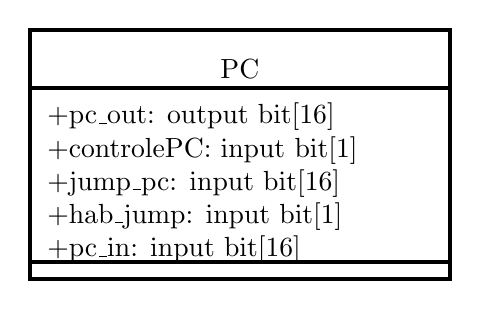
\begin{tikzpicture}
\pgftransformxscale{1.000000}
\pgftransformyscale{-1.000000}
\definecolor{dialinecolor}{rgb}{0.000000, 0.000000, 0.000000}
\pgfsetstrokecolor{dialinecolor}
\definecolor{dialinecolor}{rgb}{1.000000, 1.000000, 1.000000}
\pgfsetfillcolor{dialinecolor}
\pgfsetlinewidth{0.100000\du}
\pgfsetdash{}{0pt}
\definecolor{dialinecolor}{rgb}{1.000000, 1.000000, 1.000000}
\pgfsetfillcolor{dialinecolor}
\fill (8.750000\du,4.350000\du)--(8.750000\du,5.750000\du)--(18.875000\du,5.750000\du)--(18.875000\du,4.350000\du)--cycle;
\definecolor{dialinecolor}{rgb}{0.000000, 0.000000, 0.000000}
\pgfsetstrokecolor{dialinecolor}
\draw (8.750000\du,4.350000\du)--(8.750000\du,5.750000\du)--(18.875000\du,5.750000\du)--(18.875000\du,4.350000\du)--cycle;
% setfont left to latex
\definecolor{dialinecolor}{rgb}{0.000000, 0.000000, 0.000000}
\pgfsetstrokecolor{dialinecolor}
\node at (13.812500\du,5.300000\du){PC};
\definecolor{dialinecolor}{rgb}{1.000000, 1.000000, 1.000000}
\pgfsetfillcolor{dialinecolor}
\fill (8.750000\du,5.750000\du)--(8.750000\du,9.950000\du)--(18.875000\du,9.950000\du)--(18.875000\du,5.750000\du)--cycle;
\definecolor{dialinecolor}{rgb}{0.000000, 0.000000, 0.000000}
\pgfsetstrokecolor{dialinecolor}
\draw (8.750000\du,5.750000\du)--(8.750000\du,9.950000\du)--(18.875000\du,9.950000\du)--(18.875000\du,5.750000\du)--cycle;
% setfont left to latex
\definecolor{dialinecolor}{rgb}{0.000000, 0.000000, 0.000000}
\pgfsetstrokecolor{dialinecolor}
\node[anchor=west] at (8.900000\du,6.450000\du){+pc\_out: output bit\ensuremath{[}16\ensuremath{]}};
% setfont left to latex
\definecolor{dialinecolor}{rgb}{0.000000, 0.000000, 0.000000}
\pgfsetstrokecolor{dialinecolor}
\node[anchor=west] at (8.900000\du,7.250000\du){+controlePC: input bit\ensuremath{[}1\ensuremath{]}};
% setfont left to latex
\definecolor{dialinecolor}{rgb}{0.000000, 0.000000, 0.000000}
\pgfsetstrokecolor{dialinecolor}
\node[anchor=west] at (8.900000\du,8.050000\du){+jump\_pc: input bit\ensuremath{[}16\ensuremath{]}};
% setfont left to latex
\definecolor{dialinecolor}{rgb}{0.000000, 0.000000, 0.000000}
\pgfsetstrokecolor{dialinecolor}
\node[anchor=west] at (8.900000\du,8.850000\du){+hab\_jump: input bit\ensuremath{[}1\ensuremath{]}};
% setfont left to latex
\definecolor{dialinecolor}{rgb}{0.000000, 0.000000, 0.000000}
\pgfsetstrokecolor{dialinecolor}
\node[anchor=west] at (8.900000\du,9.650000\du){+pc\_in: input bit\ensuremath{[}16\ensuremath{]}};
\definecolor{dialinecolor}{rgb}{1.000000, 1.000000, 1.000000}
\pgfsetfillcolor{dialinecolor}
\fill (8.750000\du,9.950000\du)--(8.750000\du,10.350000\du)--(18.875000\du,10.350000\du)--(18.875000\du,9.950000\du)--cycle;
\definecolor{dialinecolor}{rgb}{0.000000, 0.000000, 0.000000}
\pgfsetstrokecolor{dialinecolor}
\draw (8.750000\du,9.950000\du)--(8.750000\du,10.350000\du)--(18.875000\du,10.350000\du)--(18.875000\du,9.950000\du)--cycle;
\end{tikzpicture}
